\documentclass{standalone}
\usepackage{circuitikz}
\begin{document}
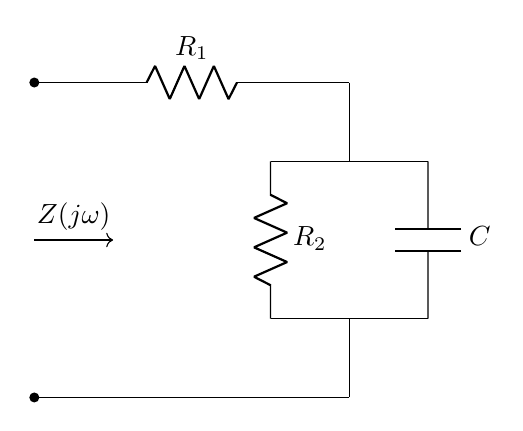
\begin{tikzpicture}
  \draw (0,0) to [R, l=$R_1$, *-] (4,0);
  \draw (4,0)--(4,-1);
  \draw (4,-1)--(3,-1);
  \draw (3,-1) to [R, l=$R_2$] (3,-3);
  \draw (3,-3)--(4,-3);
  \draw (4,-3)--(4,-4);
  \draw (3,-1)--(5,-1);
  \draw (5,-1) to [C, l=$C$] (5,-3);
  \draw (5,-3)--(3,-3);
  \draw (4,-4) to [short, -*] (0,-4);
  
  % Arrow for Z(jw)
  \draw[->] (0,-2) -- (1,-2) node[midway, above] {$Z(j\omega)$};
\end{tikzpicture}
\end{document}

